\documentclass[11pt,onecolumn,titlepage,letterpaper]{article}

\usepackage{cvpr}
\usepackage{times}
\usepackage{epsfig}
\usepackage{graphicx}
\usepackage{amsmath}
\usepackage{amssymb}
\usepackage{mathtools}
\usepackage{array}
\usepackage{multirow}
\usepackage{float}

% Box for the confusion matrix
\newcommand\MyBox[2]{
	\fbox{\lower0.75cm
		\vbox to 1.7cm{\vfil
			\hbox to 1.7cm{\hfil\parbox{1.1cm}{#1#2}\hfil}
			\vfil}%
	}%
}


% Include other packages here, before hyperref.

% If you comment hyperref and then uncomment it, you should delete
% egpaper.aux before re-running latex.  (Or just hit 'q' on the first latex
% run, let it finish, and you should be clear).
\usepackage[breaklinks=true,bookmarks=false]{hyperref}

\cvprfinalcopy % *** Uncomment this line for the final submission

\def\cvprPaperID{****} % *** Enter the CVPR Paper ID here
\def\httilde{\mbox{\tt\raisebox{-.5ex}{\symbol{126}}}}


% Pages are numbered in submission mode, and unnumbered in camera-ready
%\ifcvprfinal\pagestyle{empty}\fi
\setcounter{page}{1}
\begin{document}

%%%%%%%%% TITLE
\title{Using tree-based algorithms and recursive feature elimination \\ for house sale price prediction }

\author{Julian Cabezas Pena\\
Student ID: a1785086\\
University of Adelaide, SA 5005 Australia\\
Prepared for COMP SCI 7209 Big Data Analysis and Project \\
{\tt\small julian.cabezaspena@student.adelaide.edu.au}
% For a paper whose authors are all at the same institution,
% omit the following lines up until the closing ``}''.
% Additional authors and addresses can be added with ``\and'',
% just like the second author.
% To save space, use either the email address or home page, not both
}

\maketitle
%\thispagestyle{empty}

%%%%%%%%% ABSTRACT
\begin{abstract}
Bagging and Boosting algorithms, based in decision trees, combine various weak learners to accomplish improved predictions, being some of the more used algorithms in structured databases. One bagging algorithm (Random Forest) and three Boosting algorithms (Gradient Boosting, Extreme Gradient Boosting and Categorical Boosting) were tested to predict the house sale price in the Ames, Iowa dataset, participating in the corresponding Kaggle competition. The workflow that was used began with data preparation, were one-hot encoding was used for categorical variables, and the target variable (SalePrice) was transformed using a logarithmic function. Then, recursive feature elimination was used to discard redundant or unimportant variables to tune the models using grid search. Finally, the models were trained using the train data and predictions were obtained for the test data, 6that were submitted to the Kaggle competition.
The results of this research showed that the tested models can work with a high numbers of features without loosing performance, and that parameter tuning can be relatively relevant to obtain good predictions. The best performing model in this case was Categorical Boosting (CatBoost), that accomplished a Root Mean Squared Log Error (RMSLE) of 0.1269, and obtaining a the 1324 position in the Kaggle leaderboard (top 27\%), showing the capabilities and potential this new model, even without fine parameter tuning.
\end{abstract}

%%%%%%%%% BODY TEXT
\section{Introduction}

In the field of pattern recognition and machine learning, regression problems are one of the most common tasks. In these kind of problems, an algorithm takes a vector $X$ as input, producing one or more continuous vectors as output. When in the training phase the algorithm takes examples of input vectors along with their corresponding target variable, it is called supervised learning \cite{Bishop2006}. 

Among machine learning tools, decision trees are some of the most common ones. This tool can be described as a sequence of binary selections, forming a tree structure \cite{Bishop2006} that generates predictions according to the end nodes of the tree \cite{Hastie2009}. This kind of algorithm was extensively applied in the past \cite{Quinlan1986, Vapnik1995}, as they are fast to construct and produce relatively interpretable workflows, being relatively resistant to outliers in the predictor variable \cite{Hastie2009} and noisy features \cite{Quinlan1986}, what makes them ideal for data exploration. However, single decision trees are suboptimal for prediction, as they tend to overfit the results in the training data if the complexity of the trees is too high, or to underfit the data if the complexity is too small, producing inaccurate results \cite{Hastie2009}. 

The shortcomings of decision trees are often approached by using boosting or bagging algorithms. In one hand, bagging is based on the simple premise of combining the output of several weak classifiers, such as simple decision trees,to generate a most accurate "committee" result. On the other hand, bagging algorithms take advantage of methods that overfit the data, such a unpruned complex trees, by fitting the model in a bootstrapped subset of the data, to then produce an committee or average result \cite{Hastie2009}. The main difference between boosting and bagging in this case is that the base desition trees are trained in sequence, and that the new tree is a "weighted form" of the previous tree, while in bagging, each tree is trained independently from the other (parallelly) \cite{Bishop2006}

One common regression problem for supervised machine learning is the prediction of the sale price of different goods, were tree-based bagging and boosting models are commonly used \cite{Ceh2018}. More specifically, this report will apply and compare these methods to predict the house sale price based on several physical and location attributes, using the Ames, Iowa dataset.

%-------------------------------------------------------------------------


\section{Ames, Iowa house sale price dataset and competition}

The goal of this project is to predict the sale price of different houses using the data coming from the Ames, Iowa housing dataset. This dataset contains a total of 2930 observations, with a large amount of explanatory variables, that can help predict the target variable (Sale Price) of houses that were sold between 2006 and 2010. The dataset contains 79 variables that can be directly associated with the final sale price of the property, these variable are focused on the quantity and the quality of the physical characteristics of the house \cite{DeCock2011}

Of the 79 explanatory variables, 14 are discrete variables, that contain the number of elements of the house, such as the number of rooms. 19 of the 79 variables contain continuous data, that is usually related to measurements of the area or length of the different spaces of the house (garage, pool, basement, etc.). Finally, the database contains 43 discrete variables, that contain information regarding the environment of the house (e.g. type of street), overall quality of the house maintenance, or the neighbourhood where it is located \cite{DeCock2011}.

This dataset is the input data for the "House Prices: Advanced Regression Techniques" competition in the Kaggle website (\url{www.kaggle.com}), were the participants are encouraged to apply regression techniques to obtain the best possible prediction. The website provides a train and a test  dataset. The train set consists in 1460 observations, that contains the 79 explanatory variables, together with the target variable "SalePrice". The test dataset contains the explanatory variables but not the sale price. The competition takes the predictions on the test set as input, calculating the Root Mean Squared Log Error (RMSLE), that is used to rank the results in a public leaderboard.

\section{Methods}

\subsection{Data preprocessing}

When machine learning algorithms are applied, considerable performance problems can be attributed to low data quality \cite{Installe2014}. Given this background, data preprocessing was applied to increase the performance of the models.

First of all, the number of missing records were counted for each of the explanatory variables, and especial emphasis was placed on filling the missing data on 16 variables, that registered more than 1\% of missing data (Figure \ref{fig:na}). In many cases, the documentation of the database was used to create new categories according to what the missing value meant:

\begin{itemize}
	\item Pool Quality (\textit{PoolQC}): NA replaced by new category "No Pool"
	\item Miscellaneous features (\textit{PoolQC}): NA replaced by the new category "No Misc" (the house did not present any miscellaneous features)
	\item Alley (\textit{Alley}): NA replaced by the new category "No Alley" (No alley access)
	\item Fence (\textit{Fence}): NA replaced by the new category "No Fence"
	\item Fire place quality (\textit{FireplaceQu}): NA replaced by the new category "No Fireplace"
	\item Basement related features (\textit{BsmtQual, BsmtCond, BsmtExposure,BsmtFinType1,BsmtFinType2}): NA replaced by the new category "No Basement"
	\item Garage related features (\textit{GarageType, GarageFinish, GarageQual,GarageCond,GarageYrBlt}): NA replaced by the new category "No Garage"
\end{itemize}

\begin{figure}[H]
	\begin{center}
		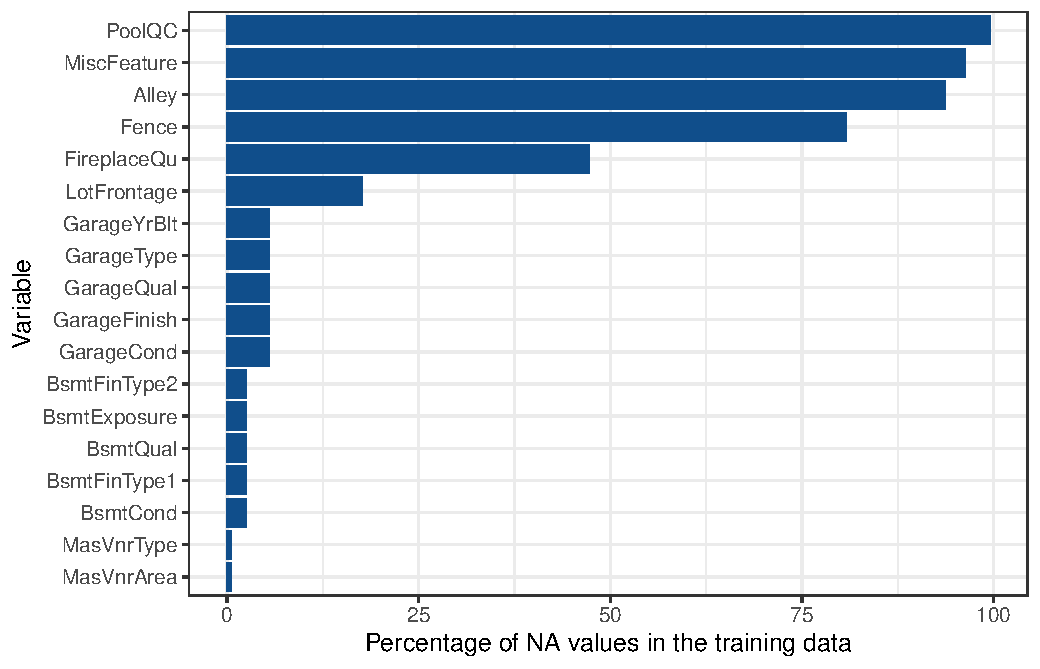
\includegraphics[width=0.8\linewidth]{NA_plot.pdf}
	\end{center}
	\caption{Percentage of missing data in the train dataset for each variable}
	\label{fig:na}
\end{figure}


In the case of the Lot frontage variable, the median of the variable per neighbourhood was used to impute the missing values. For the rest of the variables, which had less than 1\% missing data, an automatic workflow was applied: If the variable was categorical, the mode of the feature in the neighbourhood was used to replace the missing data, while in the case of numerical variables, the median of the variable in the neighbourhood was used.

Al many of implementation of the tested algorithms do not support the inclusion of categorical variables (specially the \textit{scikit-learn} implementations), a one-hot encoding was used. This process creates a new feature for each of the categories for the variable and fills it with one (1) if the category is present and zero (0) otherwise (binary encoding) \cite{Mittag2015}.  

Due to the fact that the response variable (Sale price) was highly skewed and presented extremely high values, a log transformation of the form $y = log(Saleprice + 1)$ was used to normalize the variable, as the literature indicates that it can be beneficial to increase the performance of the models \cite{Dettling2003,  Stevens2015}.

\subsection{Machine learning tools}

In order to compare the performance of different decision tree based machine learning tools, four different methods were tested, one correspond to a bagging algorithm and three to a boosting algorithm:

\textbf{Random Forest (RF)}: This bagging method was first introduced by Breiman \cite{Breiman2001b}, and consists in the a large collection of de-correlated decision trees, using a user-defined number of trees, the algorithm draws a bootstrap sample of the training data, to grow a decision tree of the subset data, selecting a random number of variables in each split, to then determine the best split point among the drawn variables, generating two child nodes. After all the trees are grown, (forming a \emph{Random Forest}), new testing data can be predicted by obtaining average of the prediction of all decision trees in the forest. \cite{Hastie2009}.

\textbf{Gradient boosting (GB)}: Very popular boosting algorithm, firstly developed by Friedman \cite{Friedman2001}. The most common application uses decision trees that are fitted sequentially, generating an additive model that combines a set of weak learners. In the case of gradient boosting, a loss function is optimized using gradient descent. The model is initialized by a single decision tree, and then in each iteration, a decision tree is grown to predict the current residuals of the model, followed by the calculation of the gradient to update the model \cite{Friedman2001, Elith2008}. This kind of models has the advantage of being able to use several loss functions \cite{Hastie2009} and are relatively robust and suitable for noisy data \cite{Friedman2001}.

\textbf{Extreme Gradient boosting (XGBoost)}: This model is similar to the gradient boosting described above, but implements an scalable system for gradient boosting, optimizing the use of resources and increasing the performance of the model. It also includes tree algorithms for sparse data and a weighted quantile method to calculate the splits in the trees on weighted datasets \cite{Chen2016}. This algorithm was included in the analysis because of its popularity and success in Kaggle challenges, as an example, 15 of the 29 challenge winning teams used XGBoost to train part or the totality of their models \cite{Chen2016}.

\textbf{Categorical Boosting (CatBoost)}: This new (2018) gradient boosting method was developed by the Yandex company, and implements a new technique of gradient boosting, according to Prokhorenjova \textit{et al} \cite{Prokhorenkova2018a}, this algorithms solves a prediction shift problem that is presented in the traditional gradient boosting algorithms, generating a new machine learning library than can outperform other state of the art machine learning libraries (a.e. XGBoost).

\subsection{Recursive feature elimination}

One of the advantages of tree-based methods is that it is easy to obtain a predictor importance measure. In the case of bagging regression (more specifically Random Forets), the decrease in the Residual Sum of Squares by the splits on the specific predictor is recorded and averaged over the produced trees \cite{James2013}. In the case of boosted regression, the importance measure is calculated using the number of times a variable is present in the node splitting of the decision trees, weighted by the error reduction caused by that node of the model, this measure is then averaged over all the trees of the model \cite{Elith2008}

In order to select the most important features for each model, and to take advantage of this variable importance characteristic, a recursive feature elimination algorithm (RFE) was applied for each of the tested methods. This iterative algorithm removes the least important feature and calculates the prediction error in each step, selecting the features that generate the best performance. According to Elith \textit{et al} \cite{Elith2008}, this procedure can be beneficial in the case of small datasets where redundant predictors can harm the performance of the model.

In order to choose the best subset of variables and avoid overfitting, a 5-fold cross validation was used to test the RFE algorithm, thus, in each fold, 80\% of the data was used to train the model with an specific number of variables (using 500 trees and default parameters), and then these models were used to predict on the remaining 20\% of the data, to then average the results in the 5 folds. This procedure was performed with all the explanatory variables, and then the most unimportant variable is removed, to repeat the algorithm until only one variable is left. The Root Mean Square Log Error (Equation 1) is calculated in each iteration and is used to pick the best subset of variables.

\begin{equation}
RMSLE = \sqrt{\frac{1}{n} \sum_{i=1}^{n} (log(p_i + 1) - log(y_i+1))^2 }
\end{equation}

where $y_i$ is the actual value and $p_i$ is the predicted value for the observation $i$.

\subsection{Model tuning}

In order to increase the prediction performance of the models, the most important hyperparameters of each model were tuned (Table \ref{table:tuning}). To pick the set of parameters to test, the documentation of the Python implementation was consulted, along with the available literature on the topic \cite{Hastie2009, James2013}

\begin{table}[H]
	\begin{center}
		\begin{tabular}{|p{4.2cm}|p{10cm}|}
			\hline
			Algorithm & Tuned parameters \\
			\hline\hline
			Random forest & $n_\mathrm{trees} = [500,1500,3000]$, $max_\mathrm{features} = [6,22,43]$ \&  $max_\mathrm{depth} = [6,10,none]$\\
			Gradient Boosting & $n_\mathrm{trees} = [500,1000,2000]$, $learning rate = {0.01,0.05,0.1}$ \& $depth = [6,8,10]$\\
			Extreme Gradient Boosting  & $n_\mathrm{trees} = [500,1000,2000]$, $learning rate = {0.01,0.05,0.1}$ \& $max_\mathrm{depth} = [3,4,5]$ \\
			Categorical Boosting & $n_\mathrm{trees} = [500,1000,2000]$, $learning rate = {0.01,0.05,0.1}$ \& $max_\mathrm{depth} = [6,8,10]$\\
			\hline
		\end{tabular}
	\end{center}
	\caption{Parameter tuning}
	\label{table:tuning}
\end{table}

To obtain the best set of parameters, a 5-fold cross validation was again implemented, picking the best combinations using the mean RMSLE on the folds.

\subsection{Model testing}

In order to asses the model performance in a real world situation, the complete train dataset was used to train the model, using the RFE selected features and the best performing (tuned) parameters, then, the test dataset was used to produce predictions with the models. These predictions were submitted to the Kaggle website of the competition (\url{https://www.kaggle.com/c/house-prices-advanced-regression-techniques}), were a RMSLE was calculated, and a position in the leader board was given to the best performing model, allowing to asses the accuracy of the model with respect to other Kaggle competitors.

\subsection{Code}

The code to reproduce this project is attached to this project, and can be also found in the GitHub repo: \url{https://github.com/juliancabezas/Big_Data_Housing_Price_Prection}, and uses mainly skikit-learn implementations \cite{Pedregosa2011} of the above mentioned methods.

As the RFE and grid search processes can take more than one hour (depending of the computing power of the equipment), the code (house\_price\_regression.py) was separated into several steps. As the steps 1 and 2 can take a great amount of time, the software stores the intermediate results into several .csv files, that are placed into the "./Intermediate\_Results" folder

\begin{itemize}
	\item Step 0: Data Preprocessing
	\item Step 1: Recursive feature Elimination
	\item Step 2: Parameter tuning (Grid Search)
	\item Step 3: Final training and testing
\end{itemize}


\section{Results and Discussion}

After the preprocessing of the dataset, the one-hot encoding of the categorical features caused the data to go from 79 to 435 explanatory variables, greatly increasing the dimensionality of the dataset, making the feature selection even more necessary. While the logarithmic conversion of the target variable (SalePrice), resulted in a distribution much more close to a normal distribution, producing the smoothness of extreme sale price values (Figure \ref{fig:log}

\begin{figure}[H]
	\begin{center}
		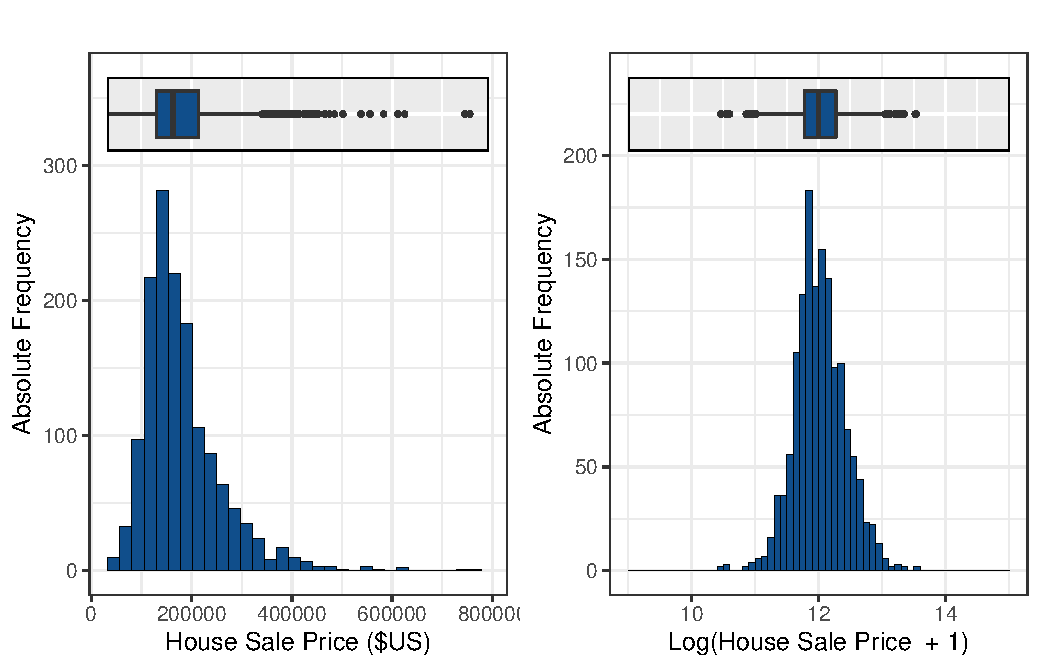
\includegraphics[width=1.0\linewidth]{2hist_saleprice.pdf}
	\end{center}
	\caption{Logarithmic conversion of the SalePrice variable. Left: original variable, right: log converted variable}
	\label{fig:log}
\end{figure}


\subsection{Feature selection}

When applying the Recursive Feature Elimination (RFE) algorithm on the 4 tested models, it is clear than the bagging and boosting algorithms presented in this research seem to perform relatively well with a high number of variables (Figure \ref{fig:rfe}), with the minimum RMSLE presented in 66 variables in the case  of the XGBoost algorithm and 184 in the case of CatBoost (Table \ref{table:rfe}). Bigger increases in the error, are observed to happen with around 30 variables in all cases, showing that a great part of the variables in the dataset are redundant to these algorithms.


\begin{figure}[H]
	\begin{center}
		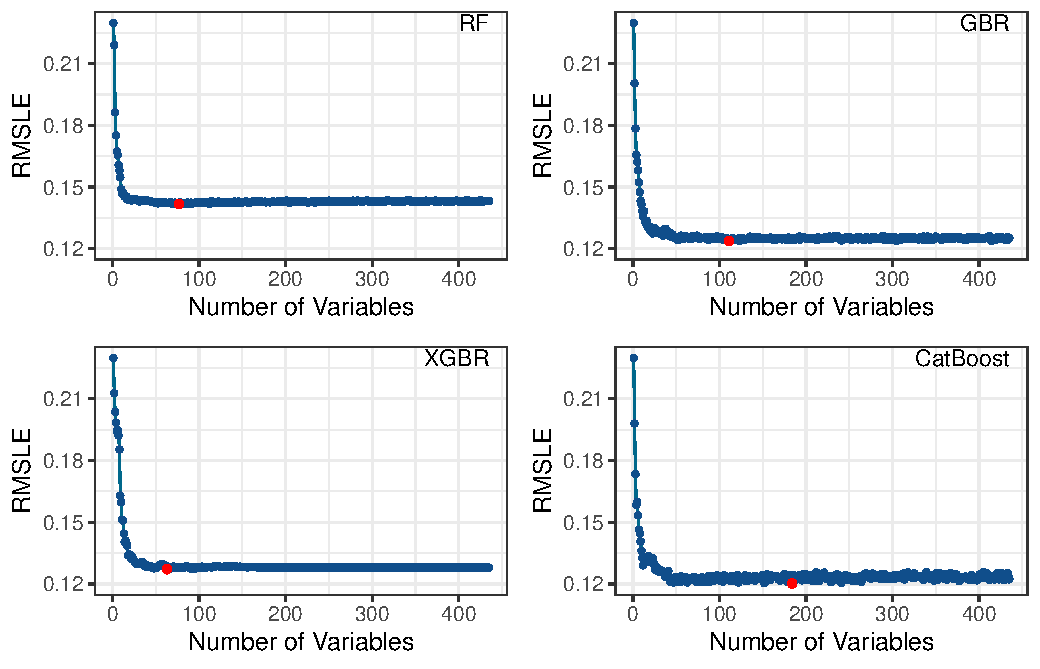
\includegraphics[width=0.8\linewidth]{RFE.pdf}
	\end{center}
	\caption{Recursive Feature Elimination (RFE) for the tested models, the red point marks the selected number of variables}
	\label{fig:rfe}
\end{figure}


\begin{table}[H]
	\begin{center}
		\begin{tabular}{|p{4.2cm}|p{4cm}|p{4cm}|}
			\hline
			Algorithm & Number of features & RMSLE (5-fold CV) \\
			\hline\hline
			Random forest & 77 & 0.1417\\
			Gradient Boosting & 111 & 0.1237 \\
			Extreme Gradient Boosting  & 66 & 0.1272\\
			Categorical Boosting & 184 & 0.1202\\
			\hline
		\end{tabular}
	\end{center}
	\caption{Recursive Feature Elimination Results}
	\label{table:rfe}
\end{table}

The RFE process allowed to generate more parsimonious models, that also decrease the computation cost to tune the models.

\subsection{Optimal parameters}

Once the variables were selected for each model, the tuning of the model generated a decrease of the RMSLE for all the models when comparing it with the previous stage, empirically, confirming the benefits of hyper-parameter tuning for the performance of the model \cite{Hastie2009}.

\begin{table}[H]
	\begin{center}
		\begin{tabular}{|p{4.2cm}|p{9cm}|p{2.5cm}|}
			\hline
			Algorithm & Tuned parameters & RMSLE (CV) \\
			\hline\hline
			Random forest & $n_\mathrm{trees} = 1500$, $max_\mathrm{features} = 22$ \&  $max_\mathrm{depth} = none$ & 0.1356\\
			Gradient Boosting & $n_\mathrm{trees} = 1000$, $learning rate = 0.1$ \& $depth = 4$ & 0.1184\\
			Extreme Gradient Boosting  & $n_\mathrm{trees} = 500$, $learning rate = 0.05$ \& $max_\mathrm{depth} = 3$ & 0.1242 \\
			Categorical Boosting & $n_\mathrm{trees} = 2000$, $learning rate = 0.1$ \& $max_\mathrm{depth} = 6$ & 0.1189\\
			\hline
		\end{tabular}
	\end{center}
	\caption{Parameter tuning}
	\label{table:tuningres}
\end{table}

\subsection{Testing results}

When getting the prediction on the test set and submitting them to Kaggle, it is possible to see that the best performing model is the newer Categorical Boosting (CatBoost) algorithm, that generates a RMSLE of 0.1269, and a classification of 1324 in the Kaggle leaderboard, positioning this implementation in the top 27\% of the ones presented in this competition (at 24 August 2020). These findings confirm the results of the tests conducted by Prokhorenkova \textit{et al} \cite{Prokhorenkova2018a}, that point out that the CatBoost algorithm can outperform other state-of-the-art algorithms such as XGBoost, even without requiring much tuning.

\begin{table}[H]
	\begin{center}
		\begin{tabular}{|p{4.2cm}|p{3cm}|p{3cm}|p{3cm}|}
			\hline
			Algorithm & RMSLE (Test set) & Kaggle Position \\
			\hline\hline
			Random forest & 0.1389 & -\\
			Gradient Boosting & 0.1372 & - \\
			Extreme Gradient Boosting  & 0.1369
			 & -\\
			Categorical Boosting & 0.1269 & 1328 of 5124\\
			\hline
		\end{tabular}
	\end{center}
	\caption{Validation and testing results}
	\label{table:test}
\end{table}

\section{Conclusion}

This project showed that decision tree based algorithms can effectively predict houses sale price, handling big quantities of variables without losing performance. The workflow presented in this report can be easily implemented for other problems, and shows that simple parameter tuning can significantly reduce the error of the model, this parameter tuning can be speeded up by feature selection, that can also increase model performance.

The best performing model was the CatBoost, being a relatively new model, it shows that can easily compete with successful models such as XGBoost. In future research, this model could be more fine tuned, archiving better results in this or other competitions.

{\small
\bibliographystyle{ieeetr}
\bibliography{library}
}

\end{document}
